
\chapter{The MVAPACK Suite for NMR Chemometrics}

\section{Introduction}

\begin{doublespace}
The biochemical laboratory procedures involved in metabolomics experiments
are potentially straightforward and inexpensive, depending on the biological
systems and pathways under study \cite{zhang:jiomic2013}. The minimal sample
handling requirements of 1D \hnmr{} NMR spectroscopy and the immense
sensitivity of multivariate bilinear factorizations such as principal component
analysis (PCA) and partial least squares (PLS) make NMR metabolic
fingerprinting especially attainable. This low barrier to entry has no doubt
contributed to the rapid recent growth of the field. Unfortunately, the data
handling tasks of NMR metabolomics are far more difficult to properly execute.
Commercial software packages available for multivariate analysis (e.g. SIMCA,
PLS Toolbox, The Unscrambler, {\it etc.}) tend to be expensive and require more
software for upstream processing and treatment of spectral data. Analysts are
thus required to first open and process NMR data in packages such as ACD/1D NMR
Manager (Advanced Chemistry Development), Mnova NMR (Mestrelabs Research) and
perform further statistical treatment in MATLAB (The Mathworks, Natick, MA), R,
or Microsoft Excel. This results in an unnecessarily cumbersome and
time-consuming data handling pipeline by forcing the analyst to pass data
between multiple software packages. As a result, the field of metabolomics
research is littered with unpublished ``in-house'' software solutions created
for processing, treating or modeling NMR datasets
\cite{viant:bbrc2003,
      verhoeckx:immpc2004,
      cloarec:anchem2005a,
      cloarec:anchem2005b,
      dieterle:anchem2006,
      kang:food2008,
      wiklund:anchem2008}. This continued reinvention of the wheel impedes
progress in the field and complicates the tasks of standardization and
communication of protocols that the metabolomics community is desperately
attempting to achieve \cite{lindon:nbiot2005,goodacre:metab2007}. Insult is
then added to injury, as these in-house solutions are far less likely than
their commercial counterparts to include proper means of validating trained
multivariate models, further contributing to the general lack of model
validation already present in the field \cite{westerhuis:metab2008a}. While
the community has released several official software packages targeted at
metabolomics
\cite{jarvis:binf2006,
      daszykowski:cils2007,
      wang:bmcb2009,
      izquierdo:bmcb2009,
      xia:nar2012,
      gaude:cmb2013,
      alonso:anchem2014}, none provide a complete, well-validated data path.
At the time of this writing, no single software package existed to bring raw
NMR data along its complete journey to validated, interpretable multivariate
models.
\\\\
These issues motivated the development of a free and open-source software
package, MVAPACK, that provides a complete pipeline of functions for NMR
chemometrics and metabolomics. MVAPACK is written in the GNU Octave
mathematical programming language \cite{eaton2008}, which is also open-source
and nearly syntactically identical to MATLAB. Thus, the installation of
GNU/Linux, Octave and MVAPACK onto a commodity workstation provides a uniform
environment in which a data analyst may truly work ``from FIDs to models'' in
a few minutes using a set of well-documented, open-source, high-level data
handling functions.
\end{doublespace}

\begin{figure}[ht!]
\begin{center}
  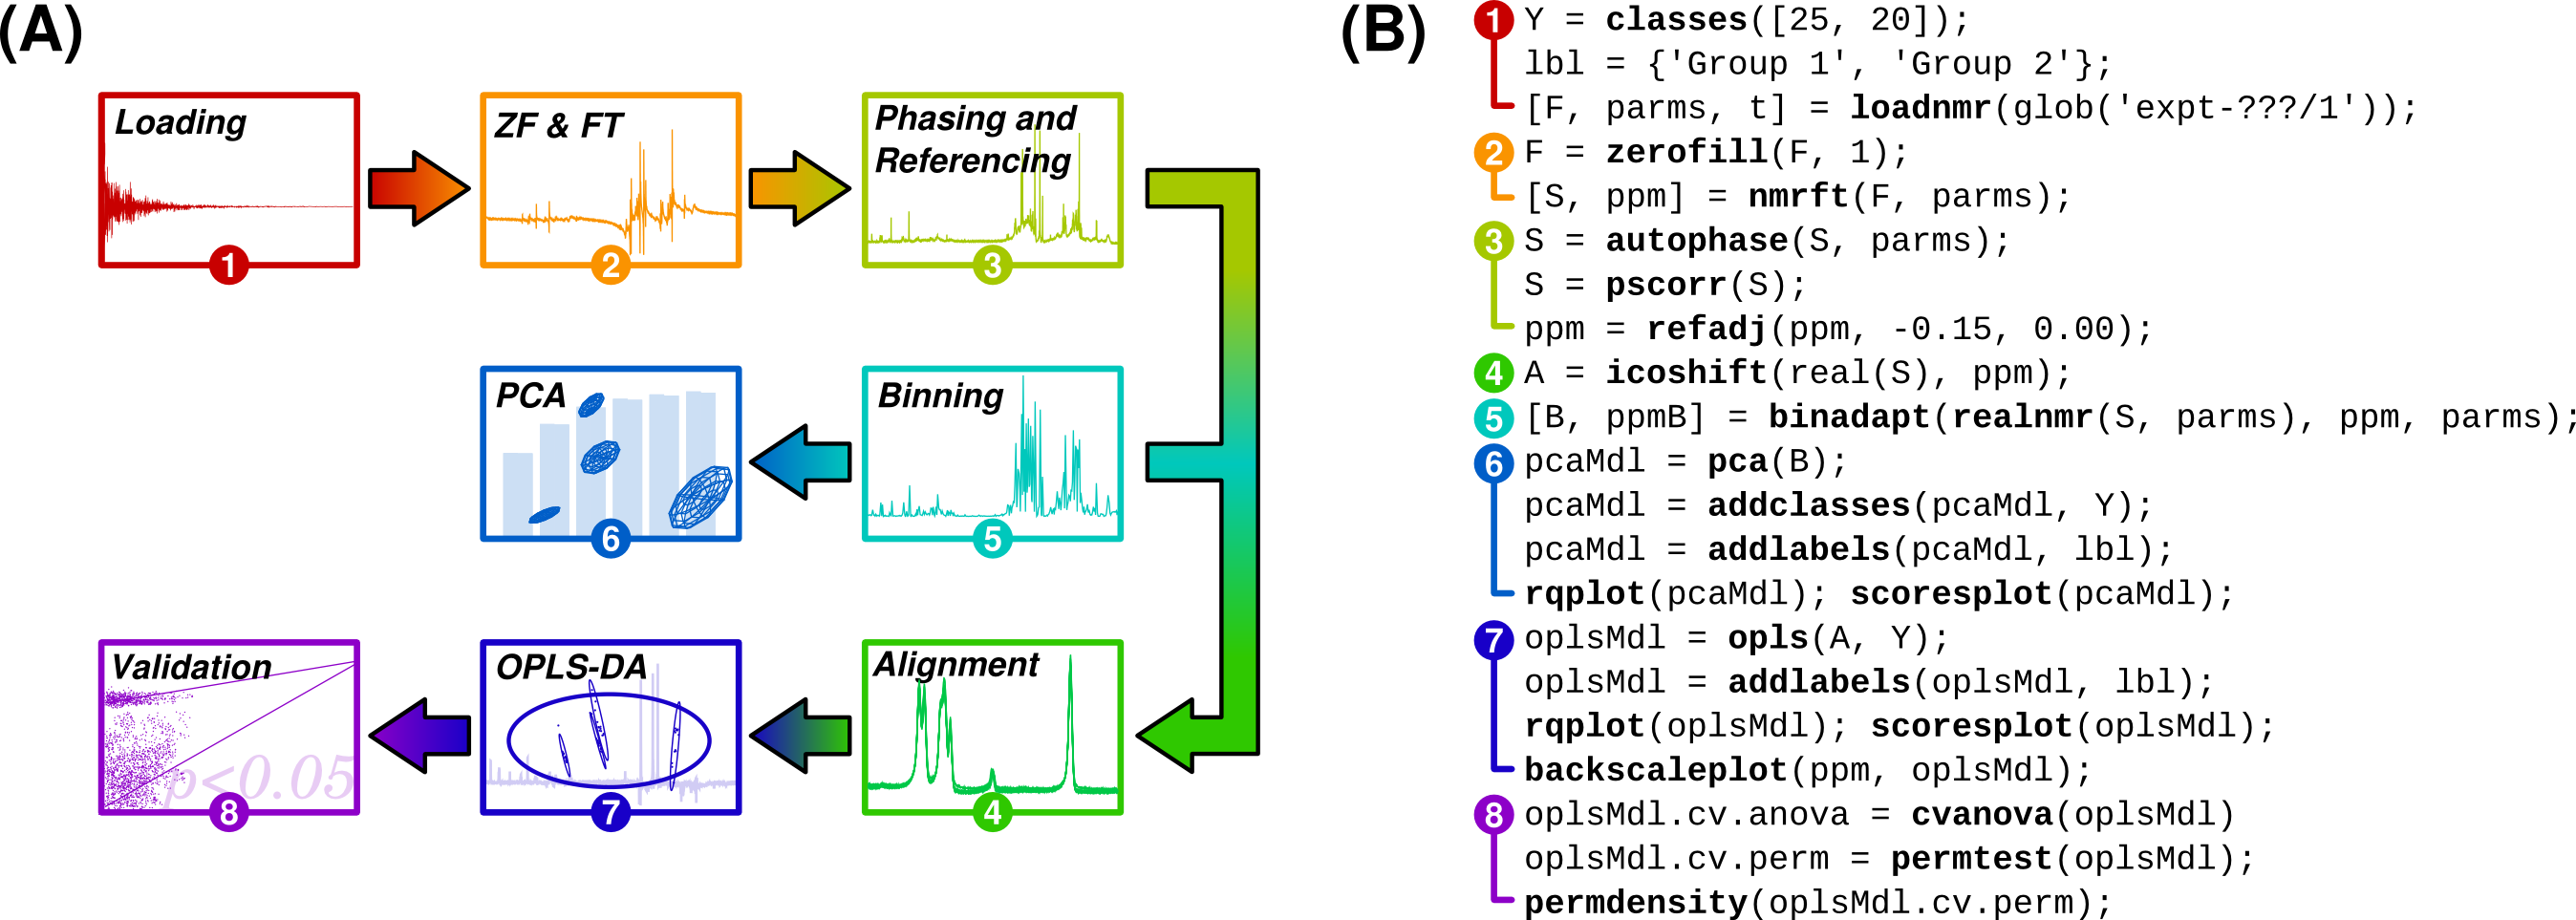
\includegraphics[width=6.5in]{figs/mvapack/01.png}
\end{center}
\caption
      [Example Data Handling Flow in MVAPACK.]{
  {\bf Example Data Handling Flow in MVAPACK.}
  \\
  A general NMR metabolic fingerprinting data handling flow diagram ({\bf A})
  and its associated minimum working example MVAPACK scripts ({\bf B}). This
  minimalistic data handling script is a simple starting point for using
  MVAPACK; much greater flexibility and functionality are present in the
  software than may be shown here. All functions in bold typeface are provided
  in MVAPACK.
}
\end{figure}

\section{Materials and Methods}

\subsection{Software Implementation}

\begin{doublespace}
The MVAPACK software package is written in GNU Octave, an open-source
mathematical programming language that uses MATLAB syntax \cite{eaton2008}.
Every function available in MVAPACK is realized as a single Octave function
file that may be examined or changed using any text editor. Most functions in
MVAPACK follow a similar input-to-output template, where an input data matrix
$\mathbf{A}$ is modified and returned as an output data matrix $\mathbf{B}$.
Other input arguments, required or optional, may accompany $\mathbf{A}$, and
extra output values may accompany $\mathbf{B}$, depending on the specific
needs of the analyst. Models produced by PCA, PLS, OPLS, LDA, MB-PCA and
MB-PLS are all similarly organized into Octave structures (i.e. ``structs'')
that all follow scalar, vector, and matrix notations of Wold et al.
\cite{wold:cils2001}. Thus, functions in MVAPACK are highly modular, often
allowing drop-in replacement of one processing, treatment or modeling method
for another by a simple change of function name and arguments. For instance,
all modeling algorithms allow the specification of a scaling method at the
time they are trained, so all available scaling functions conform to the
same interface: for any input data matrix, a scaled data matrix is returned
alongside the centering and scaling vectors used to compute the matrix.
\\\\
Data may be handled in MVAPACK in either interactive mode, in which the user
types commands into the Octave interpreter one at a time, or in batch mode,
where a complete processing scheme has been laid out in an Octave script to
be executed non-interactively. Once an ideal set of data handling steps is
determined by interactive manipulation of any given dataset, it may be
immortalized in an Octave script, thus providing documentation of procedures
and allowing for rapid recalculation of all associated results.
\\\\
Figure 4.1 illustrates a simple MVAPACK script capable of taking 1D \hnmr{} NMR
data from raw free induction decays to validated PCA and OPLS-DA models. In
section 1, a binary class matrix $\mathbf{Y}$ and an accompanying set of class
labels are built, and the time-domain raw data is loaded into the complex data
matrix $\mathbf{F}$. In section 2, the time-domain data matrix $\mathbf{F}$ is
zero-filled once and Fourier-transformed to produce the complex spectral data
matrix $\mathbf{S}$. Section 3 automatically phase corrects each spectrum in
$\mathbf{S}$, normalizes and corrects for between-spectrum phase differences,
and corrects the chemical shift abscissa to center the reference peak at $0.0$
ppm. In sections 4 and 5, data handling splits into two pathways, where
icoshift alignment \cite{savorani:jmr2010} is used to generate a data matrix
$\mathbf{A}$ fit for full-resolution OPLS-DA and AI-binning
\cite{demeyer:anchem2008} is used to generate a data matrix $\mathbf{B}$ for
PCA. In section 6, a PCA model is built and assigned classes and labels, and
a model quality plot and a scores plot are produced. In section 7, similar
functions are used to train an OPLS-DA model and produce summary plots.
Finally, section 8 performs CV-ANOVA \cite{eriksson:jchemo2008} and response
permutation \cite{westerhuis:metab2008a} significance tests to fully validate
the supervised OPLS-DA model. While Figure 4.1 is completely functional, it is
still an extremely bare-bones approach to metabolic fingerprinting. MVAPACK
provides countless other functions and schemes for handling data.
\end{doublespace}

\subsection{Feature Set}

\begin{doublespace}
The functions available in MVAPACK span the following general categories:
data loading and processing (Figure 4.1), treatment (Figure 4.2),
modeling (Figure 4.3), and validation (Figure 4.4) \cite{goodacre:metab2007}.
Specific features in each category are discussed in the following sections.
\end{doublespace}

\begin{table}[h!]
\caption{MVAPACK Processing Feature Matrix.}
\begin{center}
\begin{tabular}{l l | l l l l l l l l l l l l l l l l}
  \hline
  & &
  \rot{Topspin} &
  \rot{VnmrJ} &
  \rot{nmrPipe} &
  \rot{NMRViewJ} &
  \rot{MNova} &
  \rot{ACD/NMR} &
  \rot{Automics} &
  \rot{Chenomx} &
  \rot{KnowItAll} &
  \rot{Metabonomic} &
  \rot{MetaboAnalyst} &
  \rot{AMIX} &
  \rot{SIMCA} &
  \rot{PLS Toolbox} &
  \rot{PyChem} &
  \rot{\bf MVAPACK} \\
  \hline
  \multicolumn{2}{l|}{{\bf Loading}} & & & & & & & & & & & & & & & & \\
  & Bruker, 1D
  & * &   & * & * & * & * & * & * & * & * &   & * &   &   &   & * \\
  & Bruker, 2D
  & * &   & * & * & * & * &   &   &   &   &   &   &   &   &   & * \\
  & Varian, 1D
  &   & * & * & * & * & * & * & * & * &   &   & * &   &   &   & * \\
  \multicolumn{2}{l|}{{\bf Apodization}} & & & & & & & & & & & & & & & & \\
  & Exponential, 1D
  & * & * & * &   & * & * &   & * & * &   &   &   &   &   &   & * \\
  & Exponential, 2D
  & * & * & * &   & * & * &   &   &   &   &   &   &   &   &   & * \\
  & Gaussian, 1D
  & * & * & * &   & * & * &   &   & * &   &   &   &   &   &   & * \\
  & Gaussian, 2D
  & * & * & * &   & * & * &   &   &   &   &   &   &   &   &   & * \\
  & Sine, 1D
  & * & * & * &   & * & * &   &   &   &   &   &   &   &   &   & * \\
  & Sine, 2D
  & * & * & * &   & * & * &   &   &   &   &   &   &   &   &   & * \\
  \multicolumn{2}{l|}{{\bf Zero-filling}} & & & & & & & & & & & & & & & & \\
  & ZF, 1D
  & * & * & * &   & * & * & * & * & * &   &   &   &   &   &   & * \\
  & ZF, 2D
  & * & * & * &   & * & * &   &   &   &   &   &   &   &   &   & * \\
  \multicolumn{2}{l|}{{\bf Transforms}} & & & & & & & & & & & & & & & & \\
  & DFT, 1D
  & * & * & * &   & * & * & * & * & * & * &   &   &   &   &   & * \\
  & DFT, 2D
  & * & * & * &   & * & * &   &   &   &   &   &   &   &   &   & * \\
  & CWT, 1D
  &   &   &   &   & * &   &   &   &   &   &   &   & * &   &   & * \\
  & IST, 2D
  & * & * &   &   & * &   &   &   &   &   &   &   &   &   &   & * \\
  \multicolumn{2}{l|}{{\bf Phase correction}} & & & & & & & & & & & & & & & & \\
  & Manual, 1D
  & * & * & * &   & * & * & * & * & * & * &   & * &   &   &   & * \\
  & Manual, 2D
  & * & * & * &   & * & * &   &   &   &   &   & * &   &   &   & * \\
  & Automatic, 1D
  & * & * &   &   & * & * & * & * & * &   &   & * &   &   &   & * \\
  & Automatic, 2D
  & * & * &   &   & * & * &   &   &   &   &   &   &   &   &   & *
\end{tabular}
\end{center}
\end{table}

\subsubsection{Processing}

\begin{doublespace}
Loading of Bruker raw data is available using either a high-performance
DMX-format loading routine or nmrPipe \cite{delaglio:jbnmr1995} as a backend,
and loading of Varian data is available using an nmrPipe backend. Additionally,
data in a variety of structured text formats may be read into MVAPACK using
standard GNU Octave routines. The NMR spectral processing functions in MVAPACK
follow the traditional paradigms of NMR processing \cite{hoch1996} and include
methods for apodization, zero-filling, Fourier transformation, Iterative Soft
Thresholding (IST) reconstruction \cite{hyberts:jacs2007}, manual and automatic
phase correction
\cite{siegel:aca1981,chen:jmr2002,balacco:mrc2009}, region of interest
selection and manipulation, peak picking \cite{du:binf2006}, integration and
referencing.
\end{doublespace}

\begin{table}[h!]
\caption{MVAPACK Treatment Feature Matrix.}
\begin{center}
\begin{tabular}{l l | l l l l l l l l l l l l l l l l}
  \hline
  & &
  \rot{Topspin} &
  \rot{VnmrJ} &
  \rot{nmrPipe} &
  \rot{NMRViewJ} &
  \rot{MNova} &
  \rot{ACD/NMR} &
  \rot{Automics} &
  \rot{Chenomx} &
  \rot{KnowItAll} &
  \rot{Metabonomic} &
  \rot{MetaboAnalyst} &
  \rot{AMIX} &
  \rot{SIMCA} &
  \rot{PLS Toolbox} &
  \rot{PyChem} &
  \rot{\bf MVAPACK} \\
  \hline
  \multicolumn{2}{l|}{{\bf Binning}} & & & & & & & & & & & & & & & & \\
  & Uniform, 1D
  &   &   &   &   & * & * & * &   & * & * &   & * &   &   &   & * \\
  & Uniform, 2D
  &   &   &   &   &   & * & * &   & * &   &   & * &   &   &   & * \\
  & Optimized, 1D
  &   &   &   &   &   &   &   &   &   &   &   & * &   &   &   & * \\
  & Adaptive, 1D
  &   &   &   &   &   &   &   &   &   &   &   & * &   &   &   & * \\
  & Adaptive, 2D
  &   &   &   &   &   &   &   &   &   &   &   &   &   &   &   & * \\
  \multicolumn{2}{l|}{{\bf Alignment}} & & & & & & & & & & & & & & & & \\
  & Global
  &   &   &   &   &   &   & * &   &   &   &   &   &   &   &   & * \\
  & Interval
  &   &   &   &   &   &   & * &   &   &   &   &   &   &   &   & * \\
  \multicolumn{2}{l|}{{\bf Normalization}} & & & & & & & & & & & & & & & & \\
  & CS
  &   &   &   &   &   &   &   &   &   &   & * & * &   & * & * & * \\
  & PQ
  &   &   &   &   &   &   &   &   &   &   & * &   &   &   &   & * \\
  & HM
  &   &   &   &   &   &   &   &   &   &   &   &   &   &   &   & * \\
  & SNV
  &   &   &   &   &   &   & * &   & * & * &   & * &   & * & * & * \\
  & MSC
  &   &   &   &   &   &   & * &   & * &   &   &   &   & * & * & * \\
  & PSC
  &   &   &   &   &   &   &   &   &   &   &   &   &   &   &   & * \\
  \multicolumn{2}{l|}{{\bf Scaling}} & & & & & & & & & & & & & & & & \\
  & UV
  &   &   & * &   &   &   & * &   & * & * & * & * & * & * & * & * \\
  & Pareto
  &   &   &   &   & * &   & * &   & * & * & * &   & * &   &   & * \\
  & Range
  &   &   &   &   & * &   &   &   & * & * & * &   & * &   &   & * \\
  & Level
  &   &   &   &   & * &   &   &   &   &   &   &   & * &   &   & * \\
  & VAST
  &   &   &   &   & * &   &   &   & * &   &   &   & * &   &   & *
\end{tabular}
\end{center}
\end{table}

\subsubsection{Treatment}

\begin{doublespace}
Functions for statistical data treatment in MVAPACK include binning
\cite{sousa:cils2013,demeyer:anchem2008}, alignment \cite{savorani:jmr2010},
normalization \cite{barnes:aspec1989,dieterle:anchem2006,torgrip:metab2008},
scaling \cite{vandenberg:bmcg2006}, and direct orthogonal signal correction
\cite{westerhuis:cils2001}. In addition, MVAPACK supports uniform binning
and AI-binning (cf. Chapter 6) of third-order data tensors stored as arrays
of real matrices in Octave.
\end{doublespace}

\begin{table}[h!]
\caption{MVAPACK Modeling Feature Matrix.}
\begin{center}
\begin{tabular}{l l | l l l l l l l l l l l l l l l l}
  \hline
  & &
  \rot{Topspin} &
  \rot{VnmrJ} &
  \rot{nmrPipe} &
  \rot{NMRViewJ} &
  \rot{MNova} &
  \rot{ACD/NMR} &
  \rot{Automics} &
  \rot{Chenomx} &
  \rot{KnowItAll} &
  \rot{Metabonomic} &
  \rot{MetaboAnalyst} &
  \rot{AMIX} &
  \rot{SIMCA} &
  \rot{PLS Toolbox} &
  \rot{PyChem} &
  \rot{\bf MVAPACK} \\
  \hline
  \multicolumn{2}{l|}{{\bf Bilinear}} & & & & & & & & & & & & & & & & \\
  & PCA
  &   &   & * &   & * &   & * &   & * & * & * & * & * & * & * & * \\
  & LDA
  &   &   &   &   &   &   & * &   &   &   &   & * &   &   &   & * \\
  & PLS
  &   &   &   &   &   &   & * &   &   & * & * & * & * & * &   & * \\
  & OPLS
  &   &   &   &   &   &   &   &   &   &   &   &   & * & * &   & * \\
  \multicolumn{2}{l|}{{\bf Multiblock}} & & & & & & & & & & & & & & & & \\
  & MB-PCA
  &   &   &   &   &   &   &   &   &   &   &   &   &   & * &   & * \\
  & MB-PLS
  &   &   &   &   &   &   &   &   &   &   &   &   &   & * &   & *
\end{tabular}
\end{center}
\end{table}

\subsubsection{Modeling}

\begin{doublespace}
MVAPACK provides complete support for building PCA \cite{jolliffe2002},
LDA \cite{hardle2012}, PLS \cite{wold1993,geladi:aca1986,wold:cils2001},
OPLS \cite{trygg:jchemo2002,bylesjo:jchemo2006}, MB-PCA and MB-PLS
\cite{westerhuis:jchemo1998,smilde:jchemo2003} models from processed
and treated datasets. At the current time, only bilinear factorizations
are supported within MVAPACK.
\end{doublespace}

\begin{table}[h!]
\caption{MVAPACK Validation Feature Matrix.}
\begin{center}
\begin{tabular}{l l | l l l l l l l l l l l l l l l l}
  \hline
  & &
  \rot{Topspin} &
  \rot{VnmrJ} &
  \rot{nmrPipe} &
  \rot{NMRViewJ} &
  \rot{MNova} &
  \rot{ACD/NMR} &
  \rot{Automics} &
  \rot{Chenomx} &
  \rot{KnowItAll} &
  \rot{Metabonomic} &
  \rot{MetaboAnalyst} &
  \rot{AMIX} &
  \rot{SIMCA} &
  \rot{PLS Toolbox} &
  \rot{PyChem} &
  \rot{\bf MVAPACK} \\
  \hline
  \multicolumn{2}{l|}{{\bf Validation}} & & & & & & & & & & & & & & & & \\
  & \rsq{}, \qsq{}
  &   &   &   &   &   &   & * &   & * & * & * & * & * & * & * & * \\
  & Permutation
  &   &   &   &   &   &   &   &   &   &   & * &   & * & * &   & * \\
  & CV-ANOVA
  &   &   &   &   &   &   &   &   &   &   &   &   & * &   &   & * \\
  \multicolumn{2}{l|}{{\bf Visualization}} & & & & & & & & & & & & & & & & \\
  & 2D Scores
  &   &   &   &   & * &   & * &   & * & * & * & * & * & * & * & * \\
  & 3D Scores
  &   &   &   &   &   &   &   &   & * & * & * &   & * & * &   & * \\
  & Loadings
  &   &   &   &   & * &   & * &   & * & * & * & * & * & * & * & * \\
  & Backscaling
  &   &   &   &   &   &   &   &   &   &   &   &   &   &   &   & * \\
  & S-plot
  &   &   &   &   &   &   &   &   &   &   &   &   & * &   &   & * \\
  & SUS-plot
  &   &   &   &   &   &   &   &   &   &   &   &   & * &   &   & * \\
  & Data Ellipsoid
  &   &   &   &   &   &   &   &   &   & * & * & * & * & * &   & * \\
  & Class Ellipsoid
  &   &   &   &   &   &   &   &   &   &   &   &   &   &   &   & *
\end{tabular}
\end{center}
\end{table}

\subsubsection{Validation}

\begin{doublespace}
All PCA and MB-PCA models are validated as they are built based on the results
of a leave-one-out internal cross-validation
\cite{eastment:tech1982,eshghi:cils2014}, and all PLS, OPLS and MB-PLS models
are validated during training based on results of a Monte Carlo leave-$n$-out
internal cross-validation \cite{xu:cils2001,xu:jchemo2004}. In all cases, a
set of \rsq{} (i.e. \rsqx{} and \rsqy{}) statistics are generated to assess
how well each data and response matrix is approximated by the models, and
\qsq{} statistics are generated to describe self-consistency and predictive
ability of each data matrix in PCA and PLS models, respectively. Per-component
\rsq{} and \qsq{} statistics are utilized by MVAPACK to estimate the optimal
number of model components. Further validation of supervised models is
available in the form of CV-ANOVA \cite{eriksson:jchemo2008} and response
permutation \cite{westerhuis:metab2008a} significance testing, both of which
report $p$ values that indicate model validity.
\end{doublespace}

\section{Discussion and Conclusions}

\begin{doublespace}
This chapter presents MVAPACK, a completely free and open-source data handling
environment tailor-suited to NMR chemometrics and \hnmr{} NMR and MS metabolic
fingerprinting applications. Unlike data handling chains composed of multiple
commercial software packages, MVAPACK is free to use, modify and distribute
according to the GNU General Public License \cite{gpl3} and provides a single
consistent data handling environment. Because MVAPACK is written for GNU
Octave, researchers already familiar with MATLAB syntax will also be familiar
with MVAPACK without a considerable learning curve. Datasets and results
obtained using MVAPACK are readily saved and exhanged using GNU Octave built-in
support for the MATLAB {\it mat}-file format.
\\\\
A recent review \cite{izquierdo:pnmrs2011} of software packages targeted at
metabolomics highlights the piecemeal nature of 1D \hnmr{} NMR data handling
in the field, where no single package is capable of performing all the tasks
required by the analyst. MVAPACK addresses this need by providing a complete
pipeline that is tuned for metabolic fingerprinting. Use of MVAPACK reduces
data analysis time in metabolic fingerprinting from days to minutes, simply
by collecting all the required functions into a single scriptable environment.
In fact, the example script in Figure 4.1 would execute in under five minutes
on a modern GNU/Linux or Mac OS X computer system.
\\\\
The routine processing of {\it any} 1D and 2D NMR spectral data may be readily
done with MVAPACK, and processing routines are easily batched. The MVAPACK
scripts written to analyze the datasets in \hyperlink{chapter.3}{Chapter 3}
are composed of intuitive, modular commands that logically subdivide the script
into recognizable tasks like automatic phase correction, spectral alignment,
normalization, {\it etc}. Furthermore, aside from physical memory limitations
of the host computer, MVAPACK does not impose any limit on the number of NMR
observations that may be simultaneously handled.
\\\\
A major advantage of MVAPACK is the seamless transfer of the processed, treated
NMR data to multivariate statistical analyses. The PCA, PLS, OPLS and LDA
bilinear modeling algorithms, now ubiquitous in the metabolomics community,
are all implemented in MVAPACK using a consistent under-the-hood framework.
Model results may be visualized and interpreted using MVAPACK routines that
provide scatter, line and bar plots of model scores, loadings and validation
statistics. Critically, MVAPACK automatically ensures that {\it all} trained
models are valid using leave-one-out and Monte Carlo leave-$n$-out internal
cross-validation routines and provides further means of validating supervised
models in the form of CV-ANOVA and response permutation significance testing.
Several powerful examples of MVAPACK applied to real datasets are presented in
\hyperlink{chapter.3}{Chapter 3}. Because it implements well-established
algorithms available from peer-reviewed chemometrics literature, MVAPACK
generates identical results when compared to expensive software packages
like Umetrics SIMCA-P+.
\\\\
In short, MVAPACK provides a complete platform for NMR chemometric data
handling that is ideal for both routine handling of metabolomics datasets and
development of novel algorithms. Unlike its closed-source predecessors, the
modular, open-source design of MVAPACK readily accepts new functionality,
allowing it to grow and maintain pace with the state-of-the-art in the
chemometrics literature. MVAPACK is freely available for download at
\url{http://bionmr.unl.edu/mvapack.php}. Detailed documentation of MVAPACK,
all datasets presented in \hyperlink{chapter.3}{Chapter 3}, and the scripts
used to handle them are also available for download.
\end{doublespace}

\bibliographystyle{abbrv}
\bibliography{bworley}

